\documentclass[border=10pt]{standalone}
\usepackage{pgfplots}
\pgfplotsset{compat=1.18}

\begin{document}
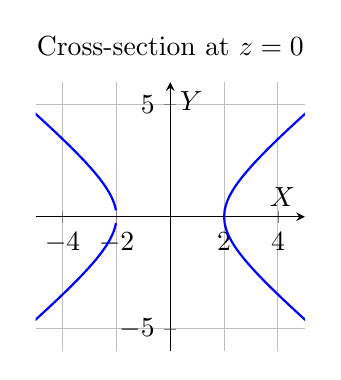
\begin{tikzpicture}
\begin{axis}[
    width=5cm,
    height=5cm,
    xlabel={$X$},
    ylabel={$Y$},
    title={Cross-section at $z=0$},
    grid=both,
    axis lines=center,
    xmin=-5, xmax=5,
    ymin=-6, ymax=6,
    domain=-6:6,
    samples=200,
]

% Hyperbola branches: x = ±sqrt(y^2 - 4)
\addplot[blue, thick, domain=2:6] {sqrt(x^2 - 4)};
\addplot[blue, thick, domain=2:6] {-sqrt(x^2 - 4)};
\addplot[blue, thick, domain=-6:-2] {sqrt(x^2 - 4)};
\addplot[blue, thick, domain=-6:-2] {-sqrt(x^2 - 4)};

\end{axis}
\end{tikzpicture}

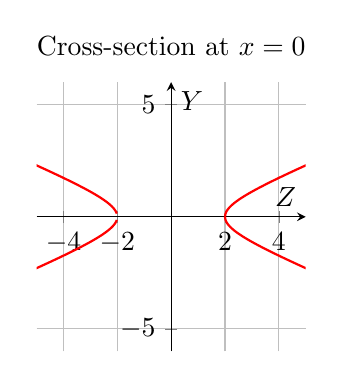
\begin{tikzpicture}
\begin{axis}[
    width=5cm,
    height=5cm,
    xlabel={$Z$},
    ylabel={$Y$},
    title={Cross-section at $x=0$},
    grid=both,
    axis lines=center,
    xmin=-5, xmax=5,
    ymin=-6, ymax=6,
    domain=-6:6,
    samples=200,
]

% Hyperbola: z = ±sqrt(y^2/4 - 1)
\addplot[red, thick, domain=2:6] {sqrt(x^2/4 - 1)};
\addplot[red, thick, domain=2:6] {-sqrt(x^2/4 - 1)};
\addplot[red, thick, domain=-6:-2] {sqrt(x^2/4 - 1)};
\addplot[red, thick, domain=-6:-2] {-sqrt(x^2/4 - 1)};

\end{axis}
\end{tikzpicture}

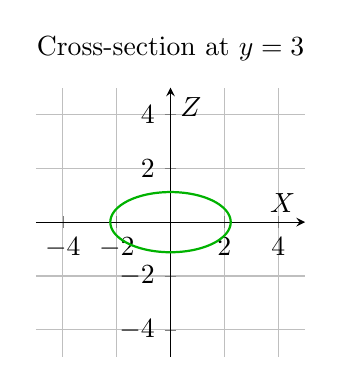
\begin{tikzpicture}
\begin{axis}[
    width=5cm,
    height=5cm,
    xlabel={$X$},
    ylabel={$Z$},
    title={Cross-section at $y=3$},
    grid=both,
    axis lines=center,
    xmin=-5, xmax=5,
    ymin=-5, ymax=5,
    domain=0:360,
    samples=200,
    axis equal,
]

% Ellipse: x^2/5 + z^2/(5/4) = 1
\addplot[green!70!black, thick] ({sqrt(5)*cos(x)}, {sqrt(5/4)*sin(x)});

\end{axis}
\end{tikzpicture}
\end{document}